% Document template suitable for use as a LaTeX master-file 
% for thesis works in University of Turku Department of Computing
%
% Technical usage guide: https://tech.utugit.fi/soft/thesis/doc/doc/overview/
% 

\documentclass[language=finnish,version=final,mainfont=none,sharelatex=false]{utuftthesis}
\setcounter{secnumdepth}{2}
\setcounter{tocdepth}{2}
\usepackage{float}
\usepackage{enumitem}
\usepackage{algpseudocode}
\usepackage{tikz}
\usepackage{subcaption}
\usepackage[caption=false]{subfig}

% Define the algorithm environment
%\makeatletter
\providecommand\textquotedblplain{%
  \bgroup\addfontfeatures{Mapping=}\char34\egroup}
\providecommand{\tabularnewline}{\\}
\floatstyle{ruled}
\newfloat{algorithm}{tbp}{loa}
\providecommand{\algorithmname}{Algoritmi}
\floatname{algorithm}{\protect\algorithmname}
%\makeatother

\addbibresource{Bibliografia.bib}

\begin{document}

\pubyear{2024}
\pubmonth{5}
\publab{Ohjelmistotekniikan laboratorio}
\publaben{Laboratory of Software Technology}
\pubtype{tkk}
\title{Polunetsintäalgoritmien esittely ja tehokkuusvertailu}
\author{Botond Ortutay}

\maketitle
\keywords{algoritmiikka, polunetsintä, graafiteoria}

\keywordsen{algorithmics, path finding, graph theory}
\begin{abstract}
\textit{Tässä tutkielmassa tarkastellaan polunetsintäalgoritmeja koneellisen 
polunetsinnän näkökulmasta. Tutkielma on kirjallisuuskatsaus, eli se perustuu 
pääosin aiheesta julkaistuun tieteelliseen kirjallisuuteen, mutta se sisältää 
pienimuotoisen tutkimuksen eräiden algoritmien mittaamisesta 
testiympäristössä. Tutkielma esittellee lukijalle joitakin 
polunetsintäalgoritmeja, sekä niiden käyttökohteita ja vertailee niiden 
tehokkuutta.}
\end{abstract}

\begin{abstracten}
\textit{This thesis examines path finding algorithms from a computing 
oriented point of view. It is a literature review, so it is mostly based on 
already published research. It also contains a small set of performance 
measurements of certain algorithms in a test environment. The thesis 
introduces the reader to a few path finding algorithms, their use cases and 
it compares their performance.}
\end{abstracten}



% mandatory
\tableofcontents

% if you want a list of figures
\listoffigures

% if you want a list of tables
%\listoftables

% if you want a list of acronyms
\listofacronyms

% change the name if the default doesn't sound right
\renewcommand{\algorithmname}{\listingscaption}

% The thesis starts here.

\begin{comment}
To better organize things, create a new tex file for each chapter
and input it below.

Avoid using the å, ä, ö or <space> characters in referred names and
underscores \_ in file names (may break hyperref).

Good luck!
\end{comment}

\chapter{Johdanto} \label{Johdanto}

\section{Tutkielman tarkoitus}\label{tTarkoitus}
\begingroup
\itshape
\paragraph{*Suunnitelma kappaleelle 1.1:*}
\begin{itemize}
	\item Harkittu ja kiinnostava aloitus
	\item Käy lyhyesti ja yksinkertaisesti läpi seuraavat asiat:
	\begin{itemize}
		\item Polunetsintäalgoritmejä tarvitaan kun...
		\item Polunetsintä käsitteenä
		\item Miski kirjoitin kandityön juuri tästä aiheesta? (tutkielman perustelu)
	\end{itemize}
	\item Päätä kappale jotenkin näin:
\end{itemize}
"Tutkielman tarkoitus on esitellä lukijalle erilaisia polunetsintäalgoritmeja, 
sekä verrata niiden toimintaa jossakin esimerkkiympäristössä"
\endgroup

\section{Tutkimuskysymykset}\label{tutkimuskysymykset}
Tutkielmassa pyritään vastaamaan seuraaviin kysymyksiin:
\begin{enumerate}[label=\textbf{\arabic*.}]
	\item \label{tKysymys1} \textbf{Tutkimuskysymys:} Minkälaisia polunetsintäalgoritmeja on kehitetty?
	\item \label{tKysymys2} \textbf{Tutkimuskysymys:} Miten niitä voidaan käyttää käytännön sovelluksiin?
	\item \label{tKysymys3} \textbf{Tutkimuskysymys:} Miten niiden tehokkuutta voidaan mitata?
\end{enumerate}

\section{Tiedonhakumenetelmät}\label{tiedonhakuM}
Tietoa tämän tutkielman tekoon on haettu IEEE:n Xplore Digital 
Center-tietokannasta, Web of Science-tietokannasta, sekä Google 
Scholar-hakupalvelusta. Hakutuloksia rajattiin julkaisuajan mukaan niin, 
että suurin osa hakutuloksista on julkaistu vuona 2018 tai sen jälkeen. 
Myös aihepiirirajausta on käytetty. Hakusanoissa on käytetty osuvempien 
tulosten löytämiseksi Boolen operaattoreita, sekä sanakatkaisua. Alla on 
muutama esimerkki käytetyistä hakusanoista:
\begin{center}
\texttt{
	pathfinding AND (grid based OR graph theory) AND "map*"	\\
	"pathfinding" AND "video gam*"				\\
	comparing AND "pathfinding algorithms"			\\
}
\end{center}

\section{Tutkielman rakenne}\label{tRakenne}
Tutkielman luku \ref{Taustoitus} taustoittaa seuraavia lukuja. Tarkoitus on, 
että luvun \ref{Taustoitus} lukemisen jälkeen lukijalle tulisivat tutuksi 
polunetsintään liittyvät peruskäsitteet ja tausta-aiheet, jotta seuraavien 
lukujen ymmärtäminen helpottuisi. Luvussa \ref{joitainP} käydään läpi 
muutaman tunnetun polunetsinnän toiminta ja täten pyritään vastaamaan 
tutkimuskysymykseen \ref{tKysymys1} Luvussa 
\ref{algoritmienSovelluskohteita} käydään läpi joitakin 
polunetsintäalgoritmien yleisiä käyttökohteita ja pyritään vastaamaan 
tutkimuskysymykseen \ref{tKysymys2} Luvussa \ref{benchmarking} taas mitataan 
useiden eri polunetsintäalgoritmien tehokkuus eräässä esimerkkiongelmassa ja 
vertaillaan niitä tämän avulla toisiinsa. Lopussa olevassa 
yhteenvetokappaleessa \ref{yhteenveto} tulokset kootaan vielä yhteen ja 
esitetään helpommin luettavassa muodossa.

\chapter{Taustoitus} \label{Taustoitus}

\section{Polunetsintä ongelmana}\label{pOngelmana}
Polunetsintä tarkoittaa tietotekniikan kontekstissa ongelmaa, jossa halutaan 
koneellisesti löytää polku kahden etukäteen määritellyn pisteen välillä. 
Useissa polunetsinnän liittyvissä ongelmissa halutaan myös, että löydetty 
polku olisi jollain tavalla optimaalinen. Optimaalinen polku voisi 
esimerkiksi olla lyhyempi tai nopeampi kuin muut mahdolliset 
polut~\cite{MathewAndMalathy}.\par
	Jotta polunetsintäongelmia voitaisiin ratkaista koneellisesti, 
täytyy ne ensin muuttaa matemaattiseen esitysmuotoon. Polunetsintäongelmat 
voidaankin jakaa kahteen osaongelmaan: graafigeneraatioon ja 
polunetsintäalgoritmin käyttöön. Graafigene\-raatiota tarvitaan, koska polun 
löytämiseen käytetyt algoritmit toimivat tyypillisesti graafeissa. Siinä 
muutetaan polunetsintäongelman alueena toimiva maasto- tai kartta-alue 
graafimuotoiseksi rakentamalla siitä esimerkiksi luurankomalli 
(skeletonization)~\cite{ACMHindawi}. Tämä tutkielma on keskittynyt 
jälkimmäiseen ongelmaan, polunetsintäalgoritmeihin ja niiden käyttöön, eikä 
graafigeneraatiota tämän vuoksi käsitellä tutkielmassa laajemmin. \par
	Polunetsintäongelmat voidaan edelleen jakaa yksiagentillisiin 
(single-agent) ja moniagentillisiin (multi-agent) polunetsintäongelmiin. 
Yksiagentillisissa ongelmissa ongelma-alueella liikkuu vain yksi agentti, 
jolle pyritään löytämään optimaalinen polku jostain lähtöpisteestä johonkin 
päämäärään. Moniagentillisissa ongelmissa alueella liikkuvia agentteja on 
useita. Näissä kaikilla agenteilla on oma lähtöpiste ja oma päämäärä ja 
kaikille tulee löytää optimaaliset polut niin, että agentit eivät törmäile 
toisiinsa ja niiden välille ei synny reititykseen liittyviä 
konflikteja~\cite{arXivMAPF}. Näistä ongelmatyypeistä tämä tutkielma käsittelee 
pääasiassa yksiagentilliseen polunetsintään kehitettyjä 
polunetsintäalgoritmeja.

\section{Algoritmeista}\label{algoritmeista}
Tässä tutkielmassa tarkasteltavat algoritmit ovat kaksiulotteisissa 
ajoaikana muuttumattomissa graafeissa toimivia yksiagenttisia 
polunetsintäalgoritmeja, ellei toisin mainita. Nämä algoritmit voidaan jakaa 
niiden toimintaperiaatteen mukaan epäinformoituihin (uninformed), 
informoituihin (informed) ja metaheuristisiin (metaheuristic) 
hakualgoritmeihin (search algorithms)~\cite{applSciLawande}.\par
	Epäinformoidut hakualgoritmit ovat yksinkertaisia algoritmeja, jotka 
eivät ole tie\-toisia ongelma-alueensa yksityiskohdista. Näin ollen 
epäinformoidut hakualgoritmit perustuvat toimintamalliin, jossa kuljetaan 
graafissa solmukohdasta toiseen kaaria pitkin niin kauan kunnes ollaan 
löydetty polku lähtösolmusta maalisolmuun. Tätä toimintamallia sanotaan joskus 
myös sokeaksi hauksi (blind search)~\cite{applSciLawande}.\par
	Informoidut hakualgoritmit sen sijaan käyttävät ongelma-alueesta 
laskettuja tie\-toja hyväksi nopeuttaakseen ajoaikaa. Tyypillisesti tämä 
tehdään laskemalla seuraavaksi läpikäytävien solmukohtien etäisyys 
maalisolmusta käyttämällä niin kutsuttua heuristista funktiota. Näin ollen 
jokaiselle graafissa olevalle solmukohdalle $n$ saadaan laskettua sen 
kautta kulkevan polun hinta $F(n)$ käyttämällä hintafunktiota 
$F(n) = G(n) + H(n)$, jossa $G(n)$ on solmulle $n$ asti kuljettu matka 
lähtösolmusta. $H(n)$ on heuristisen funktion palauttama arvo. 
Kalliita solmukohtia ei tutkita algoritmin ajon aikana, jonka takia 
tutkittavia solmuja on sokeaan hakuun verrattuna yhteensä vähemmän ja 
algoritmi on nopeampi ajaa~\cite{applSciLawande}.\par
	A* (luetaan A-tähti tai A-star) on yksi esimerkki informoidusta 
hakualgoritmista. A* on yksi suosituimmista polunetsintäalgoritmeista 
käytännön sovelluskoh\-teissa. Tämä johtuu siitä, että A* on yksinkertainen 
toteuttaa ja se palauttaa aina optimaalisen polun, mikäli käytetään 
sopivaa heuristista funktiota~\cite{MathewAndMalathy}. Sen pohjalta on 
myös kehitetty muita polunetsintäalgoritmeja~\cite{applSciLawande}.\par
	Metaheuristiset algoritmit eivät perustu heuristisiin funktioihin tai 
solmukohtien tutkimiseen vaan ne käyttävät muunlaisia keinoja polkujen 
etsimiseen~\cite{applSciLawande}. Niitä ei käydä tässä tutkielmassa tarkemmin 
läpi.

\section{Esimerkkejä sovelluskohteista}\label{eSuovelluskohteista}
Polunetsintäongelmia joudutaan ratkomaan muun muassa videopeleissä, 
karttaoh\-jelmissa, erilaisissa simulaatioissa ja 
robotiikassa~\cite{ACMHindawi}, sekä esimerkiksi logistiikan alan 
automaatiossa ja robotisoitujen autojen kehityksessä~\cite{arXivMAPF}. 
Merkittävän suuri osa po\-lun\-etsintäongelmiin liittyvistä tutkimuksista tehdään 
nimenomaan 
videopelien~\cite{MathewAndMalathy}\cite{ACMHindawi}\cite{mazeGameTrilogi}
ja robotiikan~\cite{ACMHindawi}\cite{DelaunayVoronoiAStar} näkökulmasta.\par
	Polunetsintäongelmia esiintyy videopeleissä, koska niissä on usein 
tarve simuloida ei-pelattavien hahmojen (non-playable character, NPC) 
liikkeitä niin, että niille on määritelty lähtö- ja maalipisteet, sekä 
sallitut ja kielletyt liikkumisalueet. Kun polunetsintäalgoritmeja 
sovelletaan videopeleihin, on tärkeää, että algoritmit ovat laskennallisesti 
tehokkaita. Esimerkiksi reaaliaikaisissa strategiapeleissä 
(real-time strategy, RTS) pelaaja liikuttaa useita eri yksiköitä eri puolille 
karttaa merkitsemällä niille pisteitä joiden kautta kulkea. Näissä 
tilanteissa on pelikokemuksen kannalta tärkeää, etteivät eri yksiköille 
suoritettavat polunetsintäalgoritmit vaikuttaisi pelin 
sujuvuuteen~\cite{MathewAndMalathy}. \textcite{mazeGameTrilogi} tutkivat 
eri polunetsintäalgoritmien toimimista videopelissä, jossa pelaaja rakentaa 
valmiiksi annetuista palikoista labyrintin ja algoritmi yrittää ratkaista 
sen. Tutkimuksessa A* osoittautui tutkituista algoritmeista parhaaksi. 
Vastaavankaltainen tutkimus käydään yksityiskohtaisemmin läpi tutkielman 
luvussa \ref{benchmarking}. \par
	Videopelien lisäksi polunetsintäalgoritmeja sovelletaan myös 
karttaohjelmissa. Niissä polunetsintää käytetään reitinhakuun, joka on 
karttaohjelmien eräs päätoiminnallisuus. Reitinhakuun käytetään usein 
Dijkstran algoritmia~\cite{IOPDijkstra}, josta puhutaan tarkemmin tutkielman 
luvussa \ref{dijkstra}. Karttaohjelmissa polunetsintä on kuitenkin melko 
erilaista kuin videopeleissä. On tärkeää, että yksittäisen optimaalisen reitin 
sijasta reitinhaku palauttaa käyttäjälle useita vaihtoehtoisia ajoreittejä, 
joita generoidaan lisää ajon aikana siltä varalta, että liikenteen olosuhteet 
muuttuvat~\cite{Lanelet2}. \textcite{Lanelet2} käyvät artikkelissaan läpi 
suunnittelemansa digitaalisen kartta-alustan Lanelet2:n lähestymistapaa 
reitinhakuun. Polunetsintäalgoritmien käyttö karttaohjelmien reitinhaussa 
käydään tarkemmin läpi tutkielman luvussa \ref{karttaohjelmat}.\par
	Polunetsintää on tutkittu myös paljon robotiikan näkökulmasta. 
Robotiikassa polunetsintää joudutaan soveltamaan muun muassa kun 
kehitetään itseajavia ajoneuvoja ja tehtaassa liikkuvia 
teollisuusrobotteja~\cite{arXivMAPF}. Esimerkiksi \textcite{Lanelet2} 
pohtivat artikkelissaan muun muassa sitä, miten itseajaville autoille 
voitaisiin kehittää karttapalveluita, joita ne voisivat soveltaa. 
Polunetsinnän soveltaminen robotiikassa on hyvin monipuolista, koska 
ongelmat ovat keskenään erilaisia ja lähestymistavatkin voivat olla 
erilaisia. Esimerkiksi jos polunetsintää käytetään tilanteessa, jossa 
tehtaassa liikkuu kymmeniä teollisuusrobotteja eri koh\-teisiin, niin 
polunetsintäalgoritmeja voidaan ajaa jokaisessa robotissa erikseen, tai 
keskustietokone voi välittää jokaiselle robotille polun, jotka muodostavat 
ratkaisun moniagentilliseen polunetsintäongelmaan. 
\textcite{DelaunayVoronoiAStar} esittävät artikkelissaan 
Delaunay-kolmiomittaukseen perustuvaa graafigeneraatiota ja tehostetun 
A*-algoritmin ajoa liikkuvassa robotissa. Polunetsintäalgoritmien 
soveltamista robotii\-kan sovelluksiin käydään tarkemmin läpi tutkielman 
luvussa \ref{robotiikka}.

\chapter{Joitain polunetsintäalgoritmeja}\label{joitainP}

\section{Leveyssuuntainen läpikäynti (BFS)}\label{bfs}
Leveyssuuntainen läpikäynti, eli leveyshaku (Breadth First Search, BFS) on 
epäinformoitu hakualgoritmi, joka perustuu sokeaan 
hakuun~\cite{applSciLawande}. Siinä graafin solmut ryhmitellään eri tasoihin 
sen mukaan monenko kaaren kautta pitää kulkea lähtösolmusta, jotta niihin 
päästään. Lähtösolmu on tasolla 0, siihen yhdistyneet solmut tasolla 1, 
tason 1 solmuihin yhdistyneet solmut tasolla 2 ja niin edelleen. 
Leveyshaussa graafin kaikki solmut käydään läpi niin, että tarkistetaan 
onko solmussa jo käyty, onko solmu maalisolmu ja mihin solmuihin sillä on 
yhteys. Sitten tallennetaan solmu läpikäytyjen solmujen listalle ja tieto 
siitä, mitä kautta solmulle on tultu~\cite{BFSRahim}. \par
	Ajetaan \textcite{applSciLawande} perusteella 
kirjoitetun, ohjelmalistauksen \ref{BFSEsim} mukaista BFS-algoritmia graafissa 
\ref{refGraf}. Asetetaan lähtösolmuksi G ja maalisolmuksi P. Oletetaan, että 
algoritmille syötetty graafidata on aakkosjärjestyksessä, jonka takia 
algoritmi käy läpi solmuja aakkosten mukaan. Tasoksi 0 asetetaan lähtösolmu G. 
Tason 1 muodostavat siihen yhteydessä olevat solut E, J ja L. Tason 2 soluja 
ovat tason 1 soluissa kiinni olevat solut, eli B, H ja O. Solmua G ei 
huomioida, koska siellä on jo käyty. Joitain solmuja voidaan kuitenkin käydä 
läpi useasti, jos niihin on useampi polku. Algoritmin ajo graafissa 
\ref{refGraf} johtaa kuvan \ref{refBFS} lopputulokseen, jossa on käyty läpi 
syaaninväriset kaaret ja löydetty punaisella merkitty polku G-E-H-K-P. \par
	Ohjelmalistauksen \ref{BFSEsim} algoritmi lopettaa etsinnän 
löydettyään yhden polun, mutta jos algoritmiin ei lisätä tätä lopetusehdoksi, 
niin algoritmi käy läpi kaikki solmut ja kaaret ja löytää kaikki mahdolliset 
polut~\cite{BFSRahim}. Haittapuoliin kuuluu suuri muistinkulutus tallennettujen 
polkujen lukumäärän takia~\cite{BFSRahim}, sekä pitkä 
ajoaika~\cite{mazeGameTrilogi}. Nämä voidaan huomata myös syaaninväristen 
kaarten suuresta määrästä.

\begin{figure}
	\begin{subfigure}[b]{0.3\textwidth}
		\centering
		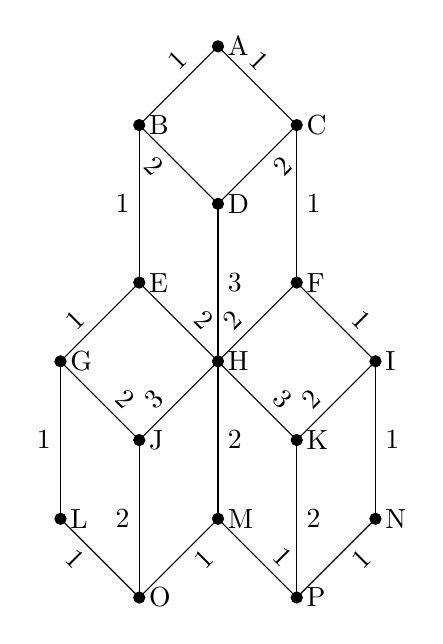
\begin{tikzpicture}[main/.style = {draw, circle}] 
		%Pisteet
		\filldraw[black] (0,6) circle (2pt) node[anchor=west]{A};
		\filldraw[black] (-1,5) circle (2pt) node[anchor=west]{B};
		\filldraw[black] (1,5) circle (2pt) node[anchor=west]{C};
		\filldraw[black] (0,4) circle (2pt) node[anchor=west]{D};
		\filldraw[black] (-1,3) circle (2pt) node[anchor=west]{E};
		\filldraw[black] (1,3) circle (2pt) node[anchor=west]{F};
		\filldraw[black] (-2,2) circle (2pt) node[anchor=west]{G};
		\filldraw[black] (0,2) circle (2pt) node[anchor=west]{H};
		\filldraw[black] (2,2) circle (2pt) node[anchor=west]{I};
		\filldraw[black] (-1,1) circle (2pt) node[anchor=west]{J};
		\filldraw[black] (1,1) circle (2pt) node[anchor=west]{K};
		\filldraw[black] (-2,0) circle (2pt) node[anchor=west]{L};
		\filldraw[black] (0,0) circle (2pt) node[anchor=west]{M};
		\filldraw[black] (2,0) circle (2pt) node[anchor=west]{N};
		\filldraw[black] (-1,-1) circle (2pt) node[anchor=west]{O};
		\filldraw[black] (1,-1) circle (2pt) node[anchor=west]{P};
		% Janat
		\draw (0,6) -- node[midway, above left, sloped] {1} (1,5);	% AB
		\draw (0,6) -- node[midway, above right, sloped] {1} (-1,5);	% AC
		\draw (-1,5) -- node[midway, below left, sloped] {2} (0,4);	% BD
		\draw (-1,5) -- node[midway, left] {1} (-1,3);			% BE
		\draw (1,5) -- node[midway, below right, sloped] {2} (0,4);	% CD
		\draw (1,5) -- node[midway, right] {1} (1,3);			% CF
		\draw (0,4) -- node[midway, right] {3} (0,2);			% DH
		\draw (-1,3) -- node[midway, above left, sloped] {1} (-2,2);	% EG
		\draw (-1,3) -- node[midway, above right, sloped] {2} (0,2);	% EH
		\draw (1,3) -- node[midway, above left, sloped] {2} (0,2);	% FH
		\draw (1,3) -- node[midway, above right, sloped] {1} (2,2);	% FI
		\draw (-2,2) -- node[midway, above right, sloped] {2} (-1,1);	% GJ
		\draw (-2,2) -- node[midway, left] {1} (-2,0);			% GL
		\draw (0,2) -- node[midway, above left, sloped] {3} (-1,1);	% HJ
		\draw (0,2) -- node[midway, above right, sloped] {3} (1,1);	% HK
		\draw (0,2) -- node[midway, right] {2} (0,0);			% HM
		\draw (2,2) -- node[midway, above left, sloped] {2} (1,1);	% IK
		\draw (2,2) -- node[midway, right] {1} (2,0);			% IN
		\draw (-1,1) -- node[midway, left] {2} (-1,-1);			% JO
		\draw (1,1) -- node[midway, right] {2} (1,-1);			% KP
		\draw (-2,0) -- node[midway, below left, sloped] {1} (-1,-1);	% LO
		\draw (0,0) -- node[midway, below right, sloped] {1} (-1,-1);	% MO
		\draw (0,0) -- node[midway, above right, sloped] {1} (1,-1);	% MP
		\draw (2,0) -- node[midway, below right, sloped] {1} (1,-1);	% NP
		\end{tikzpicture}
		\caption{Referenssigraafi.}\label{refGraf}
	\end{subfigure}
	\hfill
	\begin{subfigure}[b]{0.3\textwidth}
		\centering
		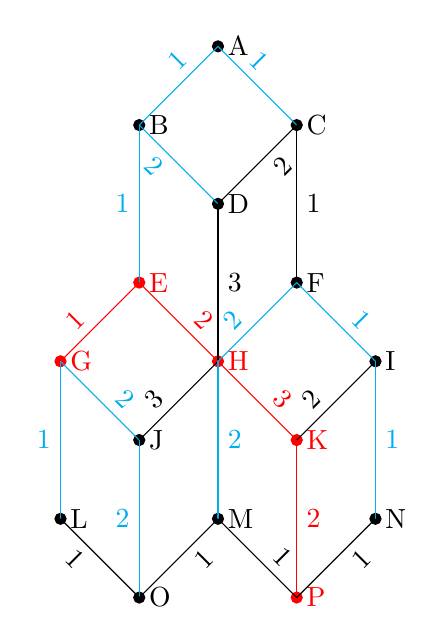
\begin{tikzpicture}[main/.style = {draw, circle}] 
		%Pisteet
		\filldraw[black] (0,6) circle (2pt) node[anchor=west]{A};
		\filldraw[black] (-1,5) circle (2pt) node[anchor=west]{B};
		\filldraw[black] (1,5) circle (2pt) node[anchor=west]{C};
		\filldraw[black] (0,4) circle (2pt) node[anchor=west]{D};
		\filldraw[red] (-1,3) circle (2pt) node[anchor=west]{E};
		\filldraw[black] (1,3) circle (2pt) node[anchor=west]{F};
		\filldraw[red] (-2,2) circle (2pt) node[anchor=west]{G};
		\filldraw[red] (0,2) circle (2pt) node[anchor=west]{H};
		\filldraw[black] (2,2) circle (2pt) node[anchor=west]{I};
		\filldraw[black] (-1,1) circle (2pt) node[anchor=west]{J};
		\filldraw[red] (1,1) circle (2pt) node[anchor=west]{K};
		\filldraw[black] (-2,0) circle (2pt) node[anchor=west]{L};
		\filldraw[black] (0,0) circle (2pt) node[anchor=west]{M};
		\filldraw[black] (2,0) circle (2pt) node[anchor=west]{N};
		\filldraw[black] (-1,-1) circle (2pt) node[anchor=west]{O};
		\filldraw[red] (1,-1) circle (2pt) node[anchor=west]{P};
		% Janat
		\draw [cyan] (0,6) -- node[midway, above left, sloped] {1} (1,5);	% AB
		\draw [cyan] (0,6) -- node[midway, above right, sloped] {1} (-1,5);	% AC
		\draw [cyan] (-1,5) -- node[midway, below left, sloped] {2} (0,4);	% BD
		\draw [cyan] (-1,5) -- node[midway, left] {1} (-1,3);			% BE
		\draw (1,5) -- node[midway, below right, sloped] {2} (0,4);	% CD
		\draw (1,5) -- node[midway, right] {1} (1,3);			% CF
		\draw (0,4) -- node[midway, right] {3} (0,2);			% DH
		\draw [red] (-1,3) -- node[midway, above left, sloped] {1} (-2,2);	% EG
		\draw [red] (-1,3) -- node[midway, above right, sloped] {2} (0,2);	% EH
		\draw [cyan] (1,3) -- node[midway, above left, sloped] {2} (0,2);	% FH
		\draw [cyan] (1,3) -- node[midway, above right, sloped] {1} (2,2);	% FI
		\draw [cyan] (-2,2) -- node[midway, above right, sloped] {2} (-1,1);	% GJ
		\draw [cyan] (-2,2) -- node[midway, left] {1} (-2,0);			% GL
		\draw (0,2) -- node[midway, above left, sloped] {3} (-1,1);	% HJ
		\draw [red] (0,2) -- node[midway, above right, sloped] {3} (1,1);	% HK
		\draw [cyan] (0,2) -- node[midway, right] {2} (0,0);			% HM
		\draw (2,2) -- node[midway, above left, sloped] {2} (1,1);	% IK
		\draw [cyan] (2,2) -- node[midway, right] {1} (2,0);			% IN
		\draw [cyan] (-1,1) -- node[midway, left] {2} (-1,-1);			% JO
		\draw [red] (1,1) -- node[midway, right] {2} (1,-1);			% KP
		\draw (-2,0) -- node[midway, below left, sloped] {1} (-1,-1);	% LO
		\draw (0,0) -- node[midway, below right, sloped] {1} (-1,-1);	% MO
		\draw (0,0) -- node[midway, above right, sloped] {1} (1,-1);	% MP
		\draw (2,0) -- node[midway, below right, sloped] {1} (1,-1);	% NP
		\end{tikzpicture}
		\caption{BFS referenssigraafissa.}\label{refBFS}
	\end{subfigure}
	\hfill
	\begin{subfigure}[b]{0.3\textwidth}
		\centering
		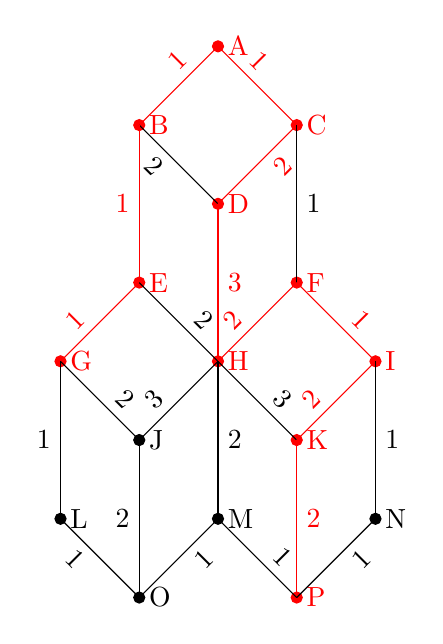
\begin{tikzpicture}[main/.style = {draw, circle}] 
		%Pisteet
		\filldraw[red] (0,6) circle (2pt) node[anchor=west]{A};
		\filldraw[red] (-1,5) circle (2pt) node[anchor=west]{B};
		\filldraw[red] (1,5) circle (2pt) node[anchor=west]{C};
		\filldraw[red] (0,4) circle (2pt) node[anchor=west]{D};
		\filldraw[red] (-1,3) circle (2pt) node[anchor=west]{E};
		\filldraw[red] (1,3) circle (2pt) node[anchor=west]{F};
		\filldraw[red] (-2,2) circle (2pt) node[anchor=west]{G};
		\filldraw[red] (0,2) circle (2pt) node[anchor=west]{H};
		\filldraw[red] (2,2) circle (2pt) node[anchor=west]{I};
		\filldraw[black] (-1,1) circle (2pt) node[anchor=west]{J};
		\filldraw[red] (1,1) circle (2pt) node[anchor=west]{K};
		\filldraw[black] (-2,0) circle (2pt) node[anchor=west]{L};
		\filldraw[black] (0,0) circle (2pt) node[anchor=west]{M};
		\filldraw[black] (2,0) circle (2pt) node[anchor=west]{N};
		\filldraw[black] (-1,-1) circle (2pt) node[anchor=west]{O};
		\filldraw[red] (1,-1) circle (2pt) node[anchor=west]{P};
		% Janat
		\draw [red] (0,6) -- node[midway, above left, sloped] {1} (1,5);	% AB
		\draw [red] (0,6) -- node[midway, above right, sloped] {1} (-1,5);	% AC
		\draw (-1,5) -- node[midway, below left, sloped] {2} (0,4);	% BD
		\draw [red] (-1,5) -- node[midway, left] {1} (-1,3);			% BE
		\draw [red] (1,5) -- node[midway, below right, sloped] {2} (0,4);	% CD
		\draw (1,5) -- node[midway, right] {1} (1,3);			% CF
		\draw [red] (0,4) -- node[midway, right] {3} (0,2);			% DH
		\draw [red] (-1,3) -- node[midway, above left, sloped] {1} (-2,2);	% EG
		\draw (-1,3) -- node[midway, above right, sloped] {2} (0,2);	% EH
		\draw [red] (1,3) -- node[midway, above left, sloped] {2} (0,2);	% FH
		\draw [red] (1,3) -- node[midway, above right, sloped] {1} (2,2);	% FI
		\draw (-2,2) -- node[midway, above right, sloped] {2} (-1,1);	% GJ
		\draw (-2,2) -- node[midway, left] {1} (-2,0);			% GL
		\draw (0,2) -- node[midway, above left, sloped] {3} (-1,1);	% HJ
		\draw (0,2) -- node[midway, above right, sloped] {3} (1,1);	% HK
		\draw (0,2) -- node[midway, right] {2} (0,0);			% HM
		\draw [red] (2,2) -- node[midway, above left, sloped] {2} (1,1);	% IK
		\draw (2,2) -- node[midway, right] {1} (2,0);			% IN
		\draw (-1,1) -- node[midway, left] {2} (-1,-1);			% JO
		\draw [red] (1,1) -- node[midway, right] {2} (1,-1);			% KP
		\draw (-2,0) -- node[midway, below left, sloped] {1} (-1,-1);	% LO
		\draw (0,0) -- node[midway, below right, sloped] {1} (-1,-1);	% MO
		\draw (0,0) -- node[midway, above right, sloped] {1} (1,-1);	% MP
		\draw (2,0) -- node[midway, below right, sloped] {1} (1,-1);	% NP
		\end{tikzpicture}
		\caption{DFS referenssigraafissa.}\label{refDFS}
	\end{subfigure}
	\caption{BFS ja DFS referenssigraafissa.}\label{refPlusBasics}
\end{figure}

\section{Syvyyssuuntainen läpikäynti (DFS)}\label{dfs}
Syvyyssuuntainen läpikäynti, eli syvyyshaku (Depth Fitst Search, DFS) on 
myös epäinformoitu sokeaan hakuun perustuva polunetsintäalgoritmi, niin kuin 
BFS~\cite{applSciLawande}. Algoritmien keskenäinen ero on  järjestys, jossa ne 
käyvät graafin solmut läpi. Siinä missä BFS muodostaa eri tasoja ja käy 
graafin läpi taso kerrallaan, DFS valitsee jokaisella solmulla yhden haaran, 
jota se lähtee seuraamaan lehtisolmuihin asti~\cite{DFSMapColoring}. 
Lehtisolmuja ovat ne, jossa minkään haaran kaari ei etene läpikäymättömään 
solmuun~\cite{DFSMapColoring}. Tällöin palataan lehdistä poispäin niin kauan, 
että löytyy haara, jossa on läpikäymättömiä solmuja, jolloin käydään sen 
haaran pohjalla. Prosessia toistetaan, kunnes polku löytyy. \par
	Ajetaan \textcite{DFSMapColoring} perusteella kirjoitetun, 
ohjelmalistauksen \ref{DFSEsim} mukaista DFS-algoritmia graafissa 
\ref{refGraf}. Ratkaistaan sama ongelma ja tehdään samat lähtöoletukset kuin 
aliluvussa \ref{bfs}. Algoritmin ajo johtaa kuvan \ref{refDFS} mukaiseen 
lopputulokseen, jossa algoritmi löysi polun G-E-B-A-C-D-H-F-I-K-P. 
Kuten kuvista näkyy, DFS-algoritmin löytämä polku on huomattavasti pidempi 
kuin BFS-algoritmin löytämä polku. BFS käy kuitenkin läpi useamman kaaren 
kuin DFS. DFS-algoritmin edut BFS:ään verrattuna ovatkin muistin ja 
suoritusajan säästyminen, koska harvempi kaari käydään 
läpi~\cite{applSciLawande}.

\section{Dijkstran algoritmi}\label{dijkstra}
Dijkstran algoritmi on Edsger Dijkstran vuonna 1956 löytämä epäinformoitu 
polunetsintäalgoritmi~\cite{applSciLawande}. Dijkstran algoritmi perustuu 
ahneuden periaatteeseen (the principle of greedy), joka tarkoittaa että joka 
suorituskerralla valitaan halvin eli kevyin saatavilla oleva 
solmu~\cite{mazeGameTrilogi}. Toisin kuin sokea haku, ahneuden periaate ei pidä 
jokaista kaarta yhtä hyvänä vaihtoehtona polunetsintäprosessissa. Jokaiselle 
kaarelle merkitään jokin hinta eli paino, jonka ahneuden periaate huomioi. Jos 
oletetaan, että graafin solmut ovat risteyksiä ja kaaret teitä, on suotavaa 
ajatella, että eri tiet eri risteyksien välissä ovat eri pituisia, vaikka tämä 
ei tieverkostosta rakennetussa graafissa näkyisikään. Voi tulla tilanteita, 
joissa oikeasti lyhyempi reitti kulkee useamman solmun läpi. Tämän takia 
graafit painotetaan. Referenssigraafissa \ref{refGraf} painot näkyvät jokaisen 
kaaren kohdalla numeroilla. \par
	Ajetaan \textcite{applSciLawande} perusteella kirjoitetun, 
ohjelmalistauksen \ref{DijkstrEsim} mukaista Dijkstran algoritmia graafissa 
\ref{refGraf}. Ratkaistaan sama ongelma ja tehdään samat lähtöoletukset kuin 
aliluvussa \ref{bfs}. Algoritmin ajo johtaa kuvan \ref{refDijkstra} mukaiseen 
lopputulokseen. Algoritmi löysi polun G-L-O-M-P. Tämä kulkee viiden 
solmukohdan läpi ja on näin mitattuna yhtä pitkä kuin reitti, jonka BFS löysi 
referenssigraafista (kuva \ref{refBFS}) ja huomattavasti lyhyempi kuin 
reitti, jonka DFS löysi referenssigraafista (kuva \ref{refDFS}). BFS ja DFS 
eivät kuitenkaan huomioi painotusta, jonka mukaan Dijkstran algoritmin 
löytämän polun hinta on 4, BFS-algoritmin 8 ja DFS-algoritmin 16. Dijkstran 
algoritmin löytämä polku on siis annetussa ongelmassa optimaalisin. Dijkstran 
algoritmia käytetäänkin usein graafiopin lyhimmän polun ongelman 
ratkaisemiseen~\cite{IOPDijkstra}. Sitä ei kuitenkaan voi käyttää 
negatiivisilla painoarvoilla~\cite{applSciLawande}. Dijkstran algoritmi on 
kuitenkin referenssiongelmassa muisti- ja suoritusaikaintensiivisempi kuin 
DFS, koska se käy läpi useampia kaaria (Dijksta 12 verrattuna DFS 10). Eri 
algoritmeja vertaillaan enemmän luvussa \ref{benchmarking}.

\begin{figure}
	\begin{subfigure}[b]{0.5\textwidth}
		\centering
		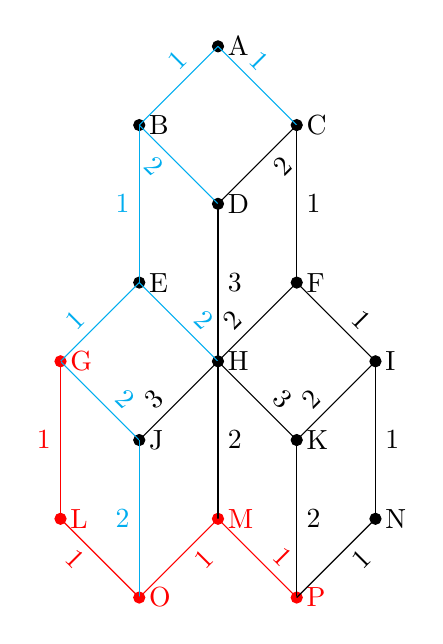
\begin{tikzpicture}[main/.style = {draw, circle}] 
		%Pisteet
		\filldraw[black] (0,6) circle (2pt) node[anchor=west]{A};
		\filldraw[black] (-1,5) circle (2pt) node[anchor=west]{B};
		\filldraw[black] (1,5) circle (2pt) node[anchor=west]{C};
		\filldraw[black] (0,4) circle (2pt) node[anchor=west]{D};
		\filldraw[black] (-1,3) circle (2pt) node[anchor=west]{E};
		\filldraw[black] (1,3) circle (2pt) node[anchor=west]{F};
		\filldraw[red] (-2,2) circle (2pt) node[anchor=west]{G};
		\filldraw[black] (0,2) circle (2pt) node[anchor=west]{H};
		\filldraw[black] (2,2) circle (2pt) node[anchor=west]{I};
		\filldraw[black] (-1,1) circle (2pt) node[anchor=west]{J};
		\filldraw[black] (1,1) circle (2pt) node[anchor=west]{K};
		\filldraw[red] (-2,0) circle (2pt) node[anchor=west]{L};
		\filldraw[red] (0,0) circle (2pt) node[anchor=west]{M};
		\filldraw[black] (2,0) circle (2pt) node[anchor=west]{N};
		\filldraw[red] (-1,-1) circle (2pt) node[anchor=west]{O};
		\filldraw[red] (1,-1) circle (2pt) node[anchor=west]{P};
		% Janat
		\draw [cyan] (0,6) -- node[midway, above left, sloped] {1} (1,5);	% AB
		\draw [cyan] (0,6) -- node[midway, above right, sloped] {1} (-1,5);	% AC
		\draw [cyan] (-1,5) -- node[midway, below left, sloped] {2} (0,4);	% BD
		\draw [cyan] (-1,5) -- node[midway, left] {1} (-1,3);			% BE
		\draw (1,5) -- node[midway, below right, sloped] {2} (0,4);	% CD
		\draw (1,5) -- node[midway, right] {1} (1,3);			% CF
		\draw (0,4) -- node[midway, right] {3} (0,2);			% DH
		\draw [cyan] (-1,3) -- node[midway, above left, sloped] {1} (-2,2);	% EG
		\draw [cyan] (-1,3) -- node[midway, above right, sloped] {2} (0,2);	% EH
		\draw (1,3) -- node[midway, above left, sloped] {2} (0,2);	% FH
		\draw (1,3) -- node[midway, above right, sloped] {1} (2,2);	% FI
		\draw [cyan] (-2,2) -- node[midway, above right, sloped] {2} (-1,1);	% GJ
		\draw [red] (-2,2) -- node[midway, left] {1} (-2,0);			% GL
		\draw (0,2) -- node[midway, above left, sloped] {3} (-1,1);	% HJ
		\draw (0,2) -- node[midway, above right, sloped] {3} (1,1);	% HK
		\draw (0,2) -- node[midway, right] {2} (0,0);			% HM
		\draw (2,2) -- node[midway, above left, sloped] {2} (1,1);	% IK
		\draw (2,2) -- node[midway, right] {1} (2,0);			% IN
		\draw [cyan] (-1,1) -- node[midway, left] {2} (-1,-1);			% JO
		\draw (1,1) -- node[midway, right] {2} (1,-1);			% KP
		\draw [red] (-2,0) -- node[midway, below left, sloped] {1} (-1,-1);	% LO
		\draw [red] (0,0) -- node[midway, below right, sloped] {1} (-1,-1);	% MO
		\draw [red] (0,0) -- node[midway, above right, sloped] {1} (1,-1);	% MP
		\draw (2,0) -- node[midway, below right, sloped] {1} (1,-1);	% NP
		\end{tikzpicture}
		\caption{Dijkstran algoritmi referenssigraafissa.}\label{refDijkstra}
	\end{subfigure}
%	\hfill
	\begin{subfigure}[b]{0.5\textwidth}
		\centering
		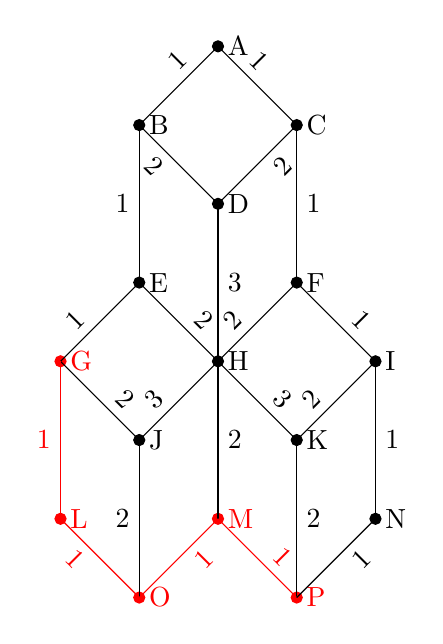
\begin{tikzpicture}[main/.style = {draw, circle}] 
		%Pisteet
		\filldraw[black] (0,6) circle (2pt) node[anchor=west]{A};
		\filldraw[black] (-1,5) circle (2pt) node[anchor=west]{B};
		\filldraw[black] (1,5) circle (2pt) node[anchor=west]{C};
		\filldraw[black] (0,4) circle (2pt) node[anchor=west]{D};
		\filldraw[black] (-1,3) circle (2pt) node[anchor=west]{E};
		\filldraw[black] (1,3) circle (2pt) node[anchor=west]{F};
		\filldraw[red] (-2,2) circle (2pt) node[anchor=west]{G};
		\filldraw[black] (0,2) circle (2pt) node[anchor=west]{H};
		\filldraw[black] (2,2) circle (2pt) node[anchor=west]{I};
		\filldraw[black] (-1,1) circle (2pt) node[anchor=west]{J};
		\filldraw[black] (1,1) circle (2pt) node[anchor=west]{K};
		\filldraw[red] (-2,0) circle (2pt) node[anchor=west]{L};
		\filldraw[red] (0,0) circle (2pt) node[anchor=west]{M};
		\filldraw[black] (2,0) circle (2pt) node[anchor=west]{N};
		\filldraw[red] (-1,-1) circle (2pt) node[anchor=west]{O};
		\filldraw[red] (1,-1) circle (2pt) node[anchor=west]{P};
		% Janat
		\draw (0,6) -- node[midway, above left, sloped] {1} (1,5);	% AB
		\draw (0,6) -- node[midway, above right, sloped] {1} (-1,5);	% AC
		\draw (-1,5) -- node[midway, below left, sloped] {2} (0,4);	% BD
		\draw (-1,5) -- node[midway, left] {1} (-1,3);			% BE
		\draw (1,5) -- node[midway, below right, sloped] {2} (0,4);	% CD
		\draw (1,5) -- node[midway, right] {1} (1,3);			% CF
		\draw (0,4) -- node[midway, right] {3} (0,2);			% DH
		\draw (-1,3) -- node[midway, above left, sloped] {1} (-2,2);	% EG
		\draw (-1,3) -- node[midway, above right, sloped] {2} (0,2);	% EH
		\draw (1,3) -- node[midway, above left, sloped] {2} (0,2);	% FH
		\draw (1,3) -- node[midway, above right, sloped] {1} (2,2);	% FI
		\draw (-2,2) -- node[midway, above right, sloped] {2} (-1,1);	% GJ
		\draw [red] (-2,2) -- node[midway, left] {1} (-2,0);			% GL
		\draw (0,2) -- node[midway, above left, sloped] {3} (-1,1);	% HJ
		\draw (0,2) -- node[midway, above right, sloped] {3} (1,1);	% HK
		\draw (0,2) -- node[midway, right] {2} (0,0);			% HM
		\draw (2,2) -- node[midway, above left, sloped] {2} (1,1);	% IK
		\draw (2,2) -- node[midway, right] {1} (2,0);			% IN
		\draw (-1,1) -- node[midway, left] {2} (-1,-1);			% JO
		\draw (1,1) -- node[midway, right] {2} (1,-1);			% KP
		\draw [red] (-2,0) -- node[midway, below left, sloped] {1} (-1,-1);	% LO
		\draw [red] (0,0) -- node[midway, below right, sloped] {1} (-1,-1);	% MO
		\draw [red] (0,0) -- node[midway, above right, sloped] {1} (1,-1);	% MP
		\draw (2,0) -- node[midway, below right, sloped] {1} (1,-1);	% NP
		\end{tikzpicture}
		\caption{A* referenssigraafissa.}\label{refAStar}
	\end{subfigure}
	\caption{Dijkstran algoritmi ja A* referenssigraafissa.}\label{DijkstraAStarFigs}
\end{figure}

\section{A*-algoritmi}\label{aStar}
A* (luetaan A-tähti tai A-star) on informoitu polunetsintäalgoritmi, joka 
täydentää Dijkstran algoritmia soveltamalla siihen heuristista 
funktiota~\cite{MathewAndMalathy}. Heuristinen funktio on jokin matemaattinen 
funktio, joka palauttaa hinnan, joka mittaa kuinka hyvä tutkittava solmu on 
ongelman ratkaisun kannalta. Kuten Dijkstran algoritmi, myös A* valitsee 
tutkittavakseen halvimmat polut ensin~\cite{DelaunayVoronoiAStar}. Dijkstran 
algoritmissa solmukohdan $n$ läpikäynnin hinnan funktio $F(n)$ on sama kuin 
lähtösolmusta solmulle $n$ johtavan halvimman polun funktio $G(n)$. Siis 
Dijkstran algoritmissa $F(n) = G(n)$ ~\cite{MathewAndMalathy}. Sen sijaan 
A*-algoritmissa yksittäisen solmun $n$ läpikäynnin hinta on 
$F(n) = G(n) + H(n)$, jossa $H(n)$ on heuristisen funktion palauttama arvo 
solmukohdalle $n$ ~\cite{DelaunayVoronoiAStar}. Dijkstran algoritmi voidaan myös 
käsittää A*-algoritmina, jossa $H(n) = 0$ ~\cite{MathewAndMalathy}.\par 
	A*-algoritmin kanssa voidaan käyttää eri heuristisia funktioita 
riippuen siitä, mikä heuristiikka toimii parhaiten tutkittavan ongelman 
kanssa. Tyypillisesti heuristiset funktiot mittaavat käytännössä tutkittavan 
solmun etäisyyttä maalisolmusta tai liikkeen suuntaa~\cite{ProcediaAStar}. 
Tyypillisiä heuristisia funktioita ovat tutkittavan solmun ja maalisolmun 
välinen Manhattan-etäisyys ja Euklidinen etäisyys~\cite{MathewAndMalathy}. 
Manhattan-etäisyys tarkoittaa kahden pisteen $P = (x_1,y_1)$ ja 
$Q = (x_2,y_2)$ välistä etäisyyttä, olettaen liikutaan vain x- ja 
y-akselien suuntaisesti~\cite{MathewAndMalathy}.

\[ d_{Manhattan}(P,Q) =  |x_1 - x_2| + |y_1 - y_2|\]
\par

	Ajetaan \textcite{MathewAndMalathy} perusteella kirjoitetun, 
ohjelmalistauksen \ref{AStarEsim} mukaista A*-algoritmia graafissa 
\ref{refGraf} ja tehdään samat lähtöoletukset kuin aliluvussa \ref{bfs}. 
Käytetään heuristisena funktiona janan pituuden kaavaa

\[ d(P) = \sqrt{(x_G-x_P)^2 + (y_G-y_P)^2} \]

jossa $P$ on $(x,y)$ muotoinen piste, ja G on maalisolmu. Algoritmin ajo 
johtaa kuvan \ref{refAStar} mukaiseen lopputulokseen. Algoritmin löytämä polku 
G-L-O-M-P on sama kuin Dijkstran algoritmin löytämä polku kuvassa 
\ref{refDijkstra}. Tähän päädyttiin kuitenkin huomattavasti nopeammin, koska 
heuristinen funktio ohjasi A*-algoritmia etsimään reittiä oikeasta suunnasta. 
\par
	A* on suosittu algoritmi käytännön sovelluksissa, koska se on 
monipuolinen, helposti toteutettava ja tehokas. Se on useimmiten se algoritmi, 
josta lähdetään liikkeelle kun polunetsintää pitää käytännössä soveltaa 
oikean elämän ongelmiin, esimerkiksi videopelikehityksessä tai 
robotiikassa~\cite{ProcediaAStar}. A* toimii myös pohjana monelle muulle 
algoritmille, koska sitä on helppo muokata ja parannella~\cite{ProcediaAStar}. 
Esimerkiksi D*-algoritmi on A*-algoritmiin perustuva polunetsintäalgoritmi, 
joka on dynaaminen, eli se kykenee reagoimaan etsintäalueen 
muuttumiseen~\cite{applSciLawande}. Hierarkkisen polunetsinnän A* (Hierarchical 
Pathfinding A*, HPA*) on hierarkkiseen polunetsintään kehitetty 
A*-variantti~\cite{applSciLawande}. Lisää hierarkkisesta polunetsinnästä 
aliluvussa \ref{hpa}. \par
	Polunetsintään liittyvissä tieteellisissä tutkimuksissa A* on myös 
suosittu lähtökohta. Usein nämä tutkimukset kehittävät jonkun A* variantin 
johonkin spesifiseen käyttötarkoitukseen~\cite{ProcediaAStar}. Esimerkiksi 
\textcite{MathewAndMalathy} käyttävät tavallista A*-algoritmia, mutta 
kehittävät siihen uudenlaisen heuristisen funktion ja 
\textcite{DelaunayVoronoiAStar} kehittävät A*-pohjaisen polunetsintäalgoritmin 
käytettäväksi robotiikassa.

\section{Hierarkkinen polunetsintä}\label{hpa}
Monet perinteiset polunetsintäalgoritmit skaalautuvat huonosti etsintäalueen 
kasvaessa ja monimutkaistuessa. Esimerkiksi \textcite{rda} demonstroivat 
artikkelissaan, kuinka A*-algoritmi kävi läpi suuren osan etsintäalueesta 
eräässä esimerkkitehtävässä. Tätä varten kehitettiin polunetsintätekniikoita 
suurille etsintäalueille. Yksi tällainen tekniikka on hierarkkinen 
polunetsintä~\cite{rda}. \par
	Hierarkkisessa polunetsinnässä etsintäalue jaetaan pienempiin 
osa-alueisiin, niin että pidetään kirjaa siitä, mitkä osa-alueet ovat 
kytköksissä toisiinsa minkäkin solmujen kautta. Tämän jälkeen 
osa-alueista muodostetaan ylemmän tason graafi~\cite{rda}. Ylemmän tason 
graafista etsitään ensin ylemmän tason polku, joka kertoo minkä 
osa-alueiden kautta varsinainen polku kulkee. Sitten kriittisten osa-alueiden 
läpi etsitään niiden kautta kulkevat polut. Nämä polut yhdistetään lopussa 
varsinaiseksi poluksi. Hierarkkisella polunetsinnällä saadaan 
yksinkertaistettua polunetsintäongelmaa abstraktion avulla ja tämä nopeuttaa 
ratkaisun löytämistä merkittävästi. Näin saadut polut eivät kuitenkaan 
välttämättä ole optimaalisia~\cite{rda}.\par
	Hierarkkisia polunetsintäalgoritmeja on monia erilaisia, esimerkiksi 
hierarkkisen polunetsinnän A* (HPA*) ja navigaatioverkkojen hierarkkisen 
polunetsinnän A* (Hierarchical pathfinding for Navigation Meshes A*, 
HNA*)~\cite{rda}. Hierarkkiset polunetsintäalgoritmit eroavat toisistaan muun 
muassa siinä, että mitä algoritmia käytetään jakamaan etsintäalue ja mitä 
polunetsintäalgoritmia käytetään polkujen löytämiseen. \textcite{rda} 
esittelevät artikkelissaan kehittämänsä alueenlöytöalgoritmin (Regions 
Discovery Algorithm, RDA), jota he vertaavat HPA*-algoritmin 
sisäänrakennettuun tapaan jakaa ruudukkomuotoinen etsintäalue alaruudukoiksi. 
Esimerkkipseudokoodi hierarkkisesta polunetsinnästä löytyy ohjelmalistauksesta 
\ref{HierarkkinenEsim}.

\chapter{Algoritmien sovelluskohteita} \label{algoritmienSovelluskohteita}

\section{Videopelit}\label{videopelit}
Monet nykyaikaiset polunetsintäalgoritmeihin liittyvät tutkimukset tehdään 
videopeliteollisuuden 
käyttöön.\cite{MathewAndMalathy}\cite{ACMHindawi}\cite{mazeGameTrilogi} 
Tämä johtuu siitä, että videopeleissä törmätään usein tilanteisiin, jossa 
NPC-hahmojen pitää liikkua videopelikartalla niin, että pelaaja ei suoraan 
itse ohjaa niitä. Tällöin pelin on itse löydettävä reitti kahden pisteen 
välille. Kun polunetsintäalgoritmeja toteutetaan videopeleissä, joudutaan 
kiinnittämään huomiota muutamiin erityisvaatimuksiin. Polunetsintäalgoritmien 
ajaminen ei saa olla liian resurssi-intensiivistä, eli sen pitää pyrkiä 
kuluttamaan tietokoneen muistia ja suoritinaikaa mahdollisimman vähän. Jotta 
resurssi-intensiivisyydeltä vältyttäisiin, voidaan löystää polun 
optimaalisuuteen liittyviä vaatimuksia, jolloin polun ei tarvitse olla enää 
lyhin mahdollinen.\cite{MathewAndMalathy} \par
	Esimerkiksi reaaliaikaisissa strategiapeleissä (real-time strategy, 
RTS) pelaaja komentaa usein eri yksiköitä eri puolelle pelialuetta 
mekitsemällä niille maalipisteitä. Näitä yksiköitä voi olla jopa satoja, 
joille pitää löytää polut suurella etsintä-alueella huomioiden mahdollisesti 
muut alueella liikkuvat yksiköt, sekä pelin säännöt siitä, että miten eri 
yksiköt käytännössä voivat liikkua.\cite{pPacman}\cite{MathewAndMalathy} 
Nämä monimutkaiset laskutoimitukset on suoritettava pelin logiikan 
vaatimalla nopeudella. Esimerkiksi videopeliyhtiö BioWare on asettanut 
säännön, jonka mukaan kaikkien pelialueella liikkuvien agenttien polunetsintä 
on kyttävä suorittamaan 1-3 ms aikana.\cite{pPacman} \par
	\textcite{pPacman} kehittivät Pathfinding-in-Pacman-projektin, jossa 
he sovelsivat polunetsintäalgoritmeja Pac-Manin kaltaiseen peliin. Pelissä 
pelihahmo liikkuu labyrintissä yrittäen kerätä pisteitä, samalla kun sitä 
jahtaavat vihollishahmoina toimivat haamut. Pelaaja voittaa kerättyään kaikki 
pisteet, ja häviää kun haamut koskevat häntä. Peli sisältää toteutukset BFS- 
ja A*-algoritmeista, sekä pelin tarkoituksiin muokatusta A*-algoritmistä, 
jota projektin raportti kutsuu Context Dependent Subgoaling A*-algoritmiksi
(kontekstiriippuvaisesti osatavoitteistava A*, CDSA*) ja ohjelmakoodi kutsuu 
subGoalAStar-algoritmiksi. CSDA* etsii polun haamulta pelaajahahmolle 
A*-algoritmilla, mikäli haamu on tarpeeksi lähellä pelaajahahmoa. Muussa 
tapauksessa CSDA* palauttaa ainoastaan suunnan, jolla haamu pääsee lähemmäs 
pelaajahahmoa. Tällä tavoin säästetään järjestelmän resursseja rajoittamalla 
tehtävien laskujen määrää. Pelissä käytetään polunetsintäalgoritmeja 
haamujen ja pelaajahahmojen välisen polun löytämiseksi ja A*- ja 
CSDA*-algoritmit käyttävät heuristiikkana Manhattan-etäisyyttä. \par
	\textcite{SturtevantDAO} vertaavat tutkimuksessaan erilaisia 
suurelle etsintäalueelle soveltuvia polunetsintätekniikoita Dragon Age: 
Origins-videopelissä (DAO) käytettyyn polunetsintään. Nämä 
polunetsintätekniikat ovat abstraktiahierarkien käyttö, parempien 
heurististen funktioiden käyttö, sekä sopimushierarkioiden (Contrarction 
Hierarchy, CH) käyttö. Abstraktihierarkia ja CH ovat hierarkisessa 
polunetsinnässä (luku \ref{hpa}) käytettäviä tapoja muodostaa ylätason 
graafi. Abstraktihierarkia muodostaa ylätason graafin niin, että 
varsinaisen etsintäalueen eri osa-alueet ovat ylätason graafin solmuja, kun 
taas CH muodostaa ylätason graafin laskemalla alkuperäisen graafin jokaiselle 
solmulle tärkeystason (importance level) ja poistamalla vähemmän tärkeät 
solmut graafista. \textcite{SturtevantDAO} osoittivat, että hierarkinen 
polunetsintä joko abstraktiohierarkiaa tai CH:ta käyttäen soveltui parhaiten 
polunetsintään DAO:n kaltaisissa videopeleissä, koska näillä menetelmillä 
käytettiin vähiten suoritinta ja muistia. DAO käyttää abstraktiohierarkiaa, 
mutta \textcite{SturtevantDAO} mainitsevat, että pelin polunetsintää olisi 
voinut tehostaa entisestään käyttämällä suurempia osa-alueita ylätason 
graafin rakentamiseen.

\section{Karttaohjelmat}\label{karttaohjelmat}
Polunetsintäalgoritmit ovat myös keskeisessä osassa karttaohjelmistoissa. 
Monet karttaohjelmat tarjoavat reitinhakupalveluita, joissa generoidaan kartan  
eri pisteiden välille reitti käyttäen polunetsintäalgoritmeja. Tämä on usein 
helppo toteuttaa, koska karttaohjelmat säilyttävät karttadataa usein 
polunetsintäalgoritmeille ideaalisessa muodossa. Esimerkiksi OpenDrive-
formaatti sisältää dataa risteyksistä ja teistä, josta kootaan 
reititysgraafi.\cite{Lanelet2} \par
	\textcite{OpenStreetMap} on yhteisön ylläpitämä avoimen lähdekoodin 
karttatietokanta, joka tarjoaa sivustollaan myös tietokannan karttadataa 
käyttävää karttaohjelmaa.\cite{OSMAbout} OpenStreetMap-karttaohjelma sisältää 
myös reitinhakumahdollisuuden. Reitinhakumahdollisuus sisältää 
reitinhakuvaihtoehdot kävelylle, pyöräilylle ja autoilulle käyttäen joko 
GraphHopperia, OSRM:ää tai Valhallaa.\cite{OpenStreetMap} \par
	Nämä ovat niin sanottuja reititysmoottoreita (routing engine), jotka 
ovat valmiita ohjelmistototeutuksia polunetsintäfunktioille.\cite{graphhopper} 
OpenStreetMapin käyttämä \textcite{graphhopper} on Javalla kirjoitettu 
reititysmoottori. Se käyttää sisäisessä toteutuksessaan Dijkstran algoritmia, 
A*-algoritmia, sekä hierarkista polunetsintää käyttäen CH-menetelmää ylätason 
graafin luomiseen ja Dijkstran algoritmiä polunetsintään. GraphHopper valitsee 
ongelmaan sopivan polunetsintämenetelmän sen asetusten perusteella.

\section{Robotiikka}\label{robotiikka}

\chapter{Eräiden algoritmien tehokkuuden tarkastelu esimerkkiongelmassa}\label{benchmarking}

Tässä tutkielmassa on verrattu kahta polunetsintäalgoritmia, Dijkstran 
algoritmia ja BFS:ää, ajamalla niitä koneellisesti monta kertaa satunnaisesti 
generoiduissa graafeissa ja tutkimalla ajautumisaikoja. Graafit on toteutettu
Boost Graph Library C++ kirjaston avulla jonka kehitti \textcite{bgl} . 
Testiohjelma ajaa algoritmit kahdessa Boost Graph Libraryn eri 
graafitoteutuksessa. Tämän tarkoitus on demonstroida graafien toteutuksen 
vaikutusta algoritmeihin. Testiohjelma itsessään on kehitetty tätä 
projektia varten ja julkaistu kokonaisuudessaan avoimen lähdekoodin jakeluun.
\cite{gt2} \par
	Testiohjelma ajaa jokaisella ajokerralla 2000 testiä, jossa jokaista 
varten generoidaan graafi $n$ solmulla ja $1,25n$ kaarella. Käytetyt 
graafikoot olivat $n=64$, $n=128$ ja $n=512$. Toteutuksen testisilmukassa 
oli kutsu, sekä BFS:lle, että Dijkstran algoritmille, sekä listatyyppisessä-, 
että matriisityyppisessä graafissa, mutta yksittäisissä testeissä 
kommentoitiin kaikki muu kuin testattava. Täten kun testattiin esimerkiksi 
Dijkstran algoritmia matriisityyppisessä graafissa, niin kaikki 
listatyyppisiin graafeihin ja BFS:ään liittyvät toimenpiteet oli kommentoitu 
pois, jolloin ne eivät vaikuta testien tuloksiin.\cite{gt2} \par

\begin{table}
\centering{}\caption{Yhteenveto testeissä mitatuista ajoista\label{tab:my-table1}}
\begin{tabular}{l|c|c|}
Graafien tyyppi ja koko (solmuja) & BFS & Dijkstran algoritmi \tabularnewline
\hline 
				Lista 64 	& 
\begin{tabular}{@{}c@{}}	Keskiarvo: 2,805 \\ Keskihajonta: 0,3972	\end{tabular} & 
\begin{tabular}{@{}c@{}}	Keskiarvo: 2,975 \\ Keskihajonta: 0,1565	\end{tabular} \tabularnewline
\hline
				Lista 128 	& 
\begin{tabular}{@{}c@{}}	Keskiarvo: 5,345 \\ Keskihajonta: 0,4766	\end{tabular} & 
\begin{tabular}{@{}c@{}}	Keskiarvo: 6,63  \\ Keskihajonta: 0,4840	\end{tabular} \tabularnewline
\hline
				Lista 512 	& 
\begin{tabular}{@{}c@{}}	Keskiarvo: 25,67 \\ Keskihajonta: 0,4714	\end{tabular} & 
\begin{tabular}{@{}c@{}}	Keskiarvo: 50,4  \\ Keskihajonta: 0,5931	\end{tabular} \tabularnewline
\hline
				Matriisi 64 	& 
\begin{tabular}{@{}c@{}}	Keskiarvo: 3,185 \\ Keskihajonta: 0,3893	\end{tabular} & 
\begin{tabular}{@{}c@{}}	Keskiarvo: 2,945 \\ Keskihajonta: 0,2286	\end{tabular} \tabularnewline
\hline 
				Matriisi 128 	& 
\begin{tabular}{@{}c@{}}	Keskiarvo: 9,49  \\ Keskihajonta: 0,5012	\end{tabular} & 
\begin{tabular}{@{}c@{}}	Keskiarvo: 8,77  \\ Keskihajonta: 0,4219	\end{tabular} \tabularnewline
\hline 
				Matriisi 512 	& 
\begin{tabular}{@{}c@{}}	Keskiarvo: 124,73 \\ Keskihajonta: 0,6156	\end{tabular} & 
\begin{tabular}{@{}c@{}}	Keskiarvo: 114,315 \\ Keskihajonta: 1,214	\end{tabular} \tabularnewline
\end{tabular}
\end{table}

Väliaikaista tekstiä, jotta näen miltä tulostaulukko näyttää takstin ympäröimänä:
Dipi diipa diipa doudou. Diipaa didi dou. Tyryry ryryryryry ryryry ryryry ry ryryryry turururu tururuu tu.
Dipi diipa diipa doudou. Diipaa didi dou. Tyryry ryryryryry ryryry ryryry ry ryryryry turururu tururuu tu.
Dipi diipa diipa doudou. Diipaa didi dou. Tyryry ryryryryry ryryry ryryry ry ryryryry turururu tururuu tu.
Dipi diipa diipa doudou. Diipaa didi dou. Tyryry ryryryryry ryryry ryryry ry ryryryry turururu tururuu tu.
Dipi diipa diipa doudou. Diipaa didi dou. Tyryry ryryryryry ryryry ryryry ry ryryryry turururu tururuu tu.
\par

Dipi diipa diipa doudou. Diipaa didi dou. Tyryry ryryryryry ryryry ryryry ry ryryryry turururu tururuu tu.
Dipi diipa diipa doudou. Diipaa didi dou. Tyryry ryryryryry ryryry ryryry ry ryryryry turururu tururuu tu.
Dipi diipa diipa doudou. Diipaa didi dou. Tyryry ryryryryry ryryry ryryry ry ryryryry turururu tururuu tu.
Dipi diipa diipa doudou. Diipaa didi dou. Tyryry ryryryryry ryryry ryryry ry ryryryry turururu tururuu tu.
Dipi diipa diipa doudou. Diipaa didi dou. Tyryry ryryryryry ryryry ryryry ry ryryryry turururu tururuu tu.


\chapter{Yhteenveto}\label{yhteenveto}

Tämän tutkielman tutkimuskysymys \ref{tKysymys1} oli selvittää minkälaisia 
polunetsintäalgoritmeja on kehitetty. Polunetsintäalgoritmit voidaan muun 
muassa jakaa yksiagentillisiin ja moniagentillisiin polunetsintäalgoritmeihin 
sen mukaan monellekko etsintäalueella liikkuvalle agentille ollaan etsimässä 
reittiä. Suurin osa tämän tutkielman luvussa \ref{joitainP} käsitellyistä 
algoritmeista on yksiagentillisia. Moniagentillisista algoritmeista puhutaan 
lähinnä luvussa \ref{robotiikka} robotiikan kontekstissa. \par
	Polunetsintäalgoritmit voidaan jakaa myös epäinformoituihin, 
informoituihin ja metaheuristisiin algoritmeihin. Näistä epäinformoidut 
algoritmit eivät ole tietoisia etsimänsä alueen yksityiskohdista, kun taas 
informoidut algoritmit voivat käyttää etsintäalueesta laskemaansa dataa 
nopeuttamaan algoritmia. Metaheuristiset algoritmit taas käyttävät muita 
keinoja kuin solmukohtien tutkimista tai heuristisia funktioita polkujen 
etsimiseen.\cite{applSciLawande} Nämä on rajattu tästä tutkielmasta pois. \par
	Näiden lisäksi on olemassa myös hierarkisia ja dynaamisia 
polunetsintäalgoritmeja. Hierarkiset polunetsintäalgoritmit luovat 
etsintäalueesta yksinkertaistetun abstraktion, jossa on helpompi ratkaista 
ongelma. Varsinaisen ongelman ratkaisu johdetaan sitten abstraktion 
ratkaisusta.\cite{rda} Hierarkisesta polunetsinnästä puhutaan tarkemmin 
luvussa \ref{hpa}. Dynaamiset algoritmit taas kykenevät reagoimaan 
etsintäalueessa tapahtuviin muutoksiin reaaliajassa. Näistä puhutaan 
pikaisesti luvussa \ref{robotiikka}. \par
	Tutkimuskysymys \ref{tKysymys2} oli selvittää miten 
polunetsintäalgoritmeja voidaan käyttää käytännön sovelluksiin. Tähän 
kysymykseen vastataan kappaleessa \ref{algoritmienSovelluskohteita}, jossa 
syvennytään tarkemmin kolmeen sovelluskohteeseen: videopeleihin, 
karttaohjelmistoihin ja robotiikkaan. \par
	Tutkimuskysymys \ref{tKysymys3} oli, että miten 
polunetsintäalgoritmien tehokkuutta voidaan mitata. Tätä varten toteutettiin 
pienimuotoinen tutkimus, joka sisälsi C++-toteutukset kahdesta algoritmista, 
joiden ajoaikoja vertailtiin. Tämän tutkimuksen tulokset ja ohjelmakoodi 
on julkaistu verkossa.\cite{gt2} Tutkimuksissa todettiin, että graafin 
tekninen toteutus vaikutti ajoaikoihin enemmän kuin käytetty algoritmi. 
Hiukan yllättäen Dijkstran algoritmi ei ollut tutkimuksessa kaikkialla 
nopeampi kuin BFS. Tämä ei vastaa muiden vastaavien kokeiden tuloksia.
\cite{mazeGameTrilogi} Muissa vastaavissa mittauksissa on mitattu ajoajan 
lisäksi löydettyjen polkujen pituutta ja laskutoimituksien lukumäärää.
\cite{mazeGameTrilogi}\cite{pPacman} \par
	Minun tekemää testiohjelmaa voisikin parantaa lisäämällä siihen 
ajoajan lisäksi muita mittareita. Lisäksi voisin jatkotutkimuksena selvittää 
miksi Dijkstran algoritmi oli testiohjelmassa tietyissä tietorakenteissa 
hitaampi kuin BFS. Mikäli se johtuu tietorakenneoperaatioiden hitauseroista 
niinkuin luulen sen johtuvan, niin saattaisi olla järkevää verrata näitä 
algoritmeja uudestaan kullekin tietorakenteelle optimoidulla algoritmilla 
geneerisen algoritmin sijasta. \par
	Tässä tutkielmassa tutustuttiin polunetsintäalgoritmeihin, sekä 
niiden käyttökohteisiin ja toteutettiin pienimuotoinen tutkimus niiden 
vertailemiseksi. Tutkimuskysymyksiin on vastattu ja mahdollisia tulevan 
tutkimisen aiheita on löydetty.


% The thesis main content ends here.

\printbibliography

\begin{comment}
Important! Create the appendix chapters with command \textbackslash appchapter\{some
name\} instead of \textbackslash chapter\{some name\} for the automagic
page counting to work!
\end{comment}

\end{document}
